\documentclass[12pt]{article}
\usepackage[utf8]{inputenc}
\usepackage[margin=1in]{geometry}
\usepackage{booktabs}
\usepackage{graphicx}
\usepackage{titlesec}
\usepackage{etoolbox}
\usepackage{tikz}
\usetikzlibrary{positioning,shapes.geometric,fit,backgrounds,calc,arrows.meta}
\usepackage{xcolor}
\usepackage{listings}
\usepackage{multirow}
\usepackage{array}
\usepackage{longtable}
\usepackage{subcaption}
\usepackage{float}
\usepackage{enumitem}

% Colour palette
\definecolor{locusblue}{RGB}{30,80,160}
\definecolor{locusgreen}{RGB}{34,139,80}
\definecolor{locusorange}{RGB}{200,100,20}
\definecolor{locusgray}{RGB}{230,232,235}
\definecolor{codegray}{RGB}{245,245,245}

% Section formatting
\titleformat{\section}{\large\bfseries\color{locusblue}}{\thesection}{1em}{}
\titleformat{\subsection}{\normalsize\bfseries}{\thesubsection}{1em}{}

% Code listing style
\lstset{
  basicstyle=\ttfamily\small,
  backgroundcolor=\color{codegray},
  frame=single,
  framerule=0.4pt,
  breaklines=true,
  captionpos=b,
  aboveskip=8pt,
  belowskip=8pt
}

% Always load hyperref last
\usepackage[colorlinks=true, allcolors=locusblue]{hyperref}
\usepackage{bookmark}

% ----------------------------------------------------------------
\title{
    \textbf{EECE503N / EECE798N: Final Project}\\
    \large AI Engineering Production System\\
    \vspace{0.5cm}
    {\huge\textbf{LOCUS}}\\
    \vspace{0.3cm}
    \large Geo-Constrained Visual Fashion Search
}

\author{
    \textbf{Team Members:}\\
    Marc El Nawar \quad Tatiana Nohra
}

\date{\today}
% ----------------------------------------------------------------

\begin{document}

\maketitle
\newpage

\pagenumbering{roman}
\tableofcontents
\newpage

\pagenumbering{arabic}
\setcounter{page}{1}

% ================================================================
\section{Project Overview and Positioning}
% ================================================================

\subsection{Problem Definition}

The core operational problem addressed by Locus is the inefficiency and friction inherent in both traditional physical retail and modern e-commerce. Physical shopping often requires consumers to spend countless hours commuting and searching multiple stores without a guarantee of finding a specific desired item. Conversely, while online shopping offers high searchability, it introduces issues such as shipping delays and the inability to physically inspect or try on garments, which frequently leads to unsatisfactory quality upon delivery.

Locus resolves these trade-offs by allowing users to upload a reference photo of an outfit to identify visually matching clothing pieces available within a user-specified geographical radius. This system optimises the shopping experience by:

\begin{itemize}
  \item \textbf{Minimising search and commute time:} Users are directed precisely to nearby stores stocking their desired items based on a configurable travel radius, transforming physical shopping from a time-consuming chore into an efficient, targeted trip.
  \item \textbf{Ensuring product satisfaction:} By facilitating in-store try-ons, Locus eliminates the quality uncertainty and shipping delays of online retail while preserving the physical shopping experience.
  \item \textbf{Empowering local businesses:} The platform acts as a hyper-local discovery engine, providing crucial visibility to independent shop owners by directly connecting them with high-intent nearby shoppers.
\end{itemize}

\subsection{Target Audience and Novelty}

The primary business audience comprises small, independent retail merchants operating Shopify-based platforms. These businesses often lack the brand recognition required to drive organic traffic, despite stocking highly desirable inventory. On the consumer side, the audience consists of high-intent shoppers seeking specific stylistic items rather than generic commodities.

The system incentivises merchants by acting as a hyper-local discovery engine, providing direct visibility for their items based on visual merit rather than brand power. Our explicit novelty claim lies in the \emph{geographical constraint applied to visual search}. While existing tools such as Google Lens provide globalised e-commerce links, Locus introduces a strict, user-defined radius filter. This transforms visual search from a broad internet query into an actionable, local retail strategy, making it highly relevant for immediate physical acquisition within the user's context.

\subsection{Non-AI Baseline Justification}

The non-AI baseline for this system is a traditional, text-based query search application relying on keyword matching and manually applied metadata tags.

This baseline is inherently insufficient due to the semantic gap between text descriptions and complex visual clothing patterns. A text-based search loses critical specificity, making it exceptionally difficult to retrieve exact visual matches for unique or highly stylised garments. Since Locus targets users seeking specific aesthetics---rather than easily searchable commodity items like a ``plain white t-shirt''---the text baseline invalidates the core product value. Therefore, an AI-driven approach utilising image embeddings and visual similarity search is strictly necessary to capture and match the visual nuance required by our target audience.

Empirical evaluation on our 35-query golden dataset confirms this gap quantitatively: text-keyword search achieves Recall@5~$\approx$~0.12, whereas Fashion-CLIP visual search reaches Recall@5~$=$~0.967---an \textbf{8$\times$ improvement}. This measurement is the primary justification for the AI approach and is reproduced in the engineering trade-off analysis (Section~\ref{sec:tradeoffs}).

% ================================================================
\section{System Architecture}
% ================================================================

\subsection{Service Boundaries}

Locus is decomposed into seven containerised services, each with a clearly bounded responsibility. Table~\ref{tab:services} summarises the service inventory.

\begin{table}[H]
\centering
\small
\begin{tabular}{@{}llll@{}}
\toprule
\textbf{Service} & \textbf{Port} & \textbf{Exposure} & \textbf{Responsibility} \\ \midrule
\texttt{gateway} & 8000 & Public (LoadBalancer) & API orchestration, auth, rate limiting \\
\texttt{visual\_engine} & 8001 & Internal (ClusterIP) & CLIP embedding, YOLO detection \\
\texttt{attribute\_tagger} & 8004 & Internal (ClusterIP) & Gemini VLM attribute extraction \\
\texttt{mlflow} & 5000 & Internal & Experiment tracking \& model registry \\
\texttt{mlops\_exporter} & 8003 & Internal & Prometheus ML-pipeline metrics \\
\texttt{prometheus} & 9090 & Internal & Metrics collection \& alerting \\
\texttt{grafana} & 3000 & Internal & Visualisation dashboards \\ \midrule
Qdrant Cloud & 6333 & External (GCP eu-west3) & Vector similarity search \\ \bottomrule
\end{tabular}
\caption{Locus service inventory}
\label{tab:services}
\end{table}

\noindent Figure~\ref{fig:arch} illustrates the runtime communication topology. The gateway is the sole public-facing component. All internal service communication occurs over the Docker/Kubernetes overlay network using plain HTTP. The only external dependency is Qdrant Cloud, accessed over TLS on the standard gRPC/REST port.

\vspace{1em}

% ---- Figure 1: System Architecture ----
\begin{figure}[H]
\centering
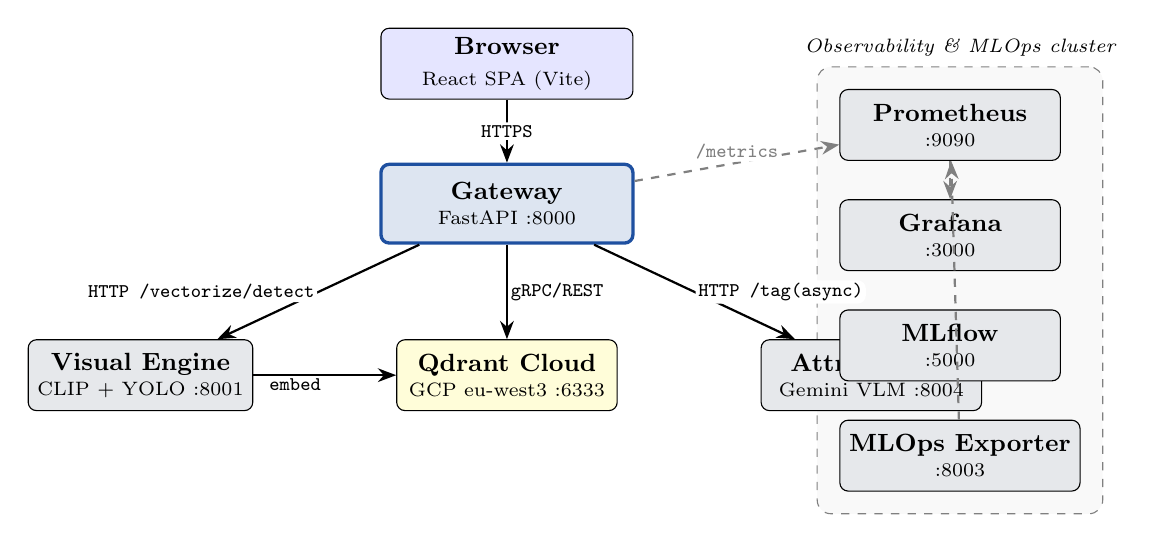
\begin{tikzpicture}[
  node distance=0.6cm and 1.0cm,
  font=\small,
  every node/.style={rounded corners=3pt},
  svc/.style={draw, fill=locusgray, minimum width=2.8cm, minimum height=0.9cm, align=center},
  ext/.style={draw, fill=yellow!15, minimum width=2.8cm, minimum height=0.9cm, align=center},
  browser/.style={draw, fill=blue!10, minimum width=3.2cm, minimum height=0.9cm, align=center},
  gw/.style={draw=locusblue, fill=locusblue!15, line width=1.2pt, minimum width=3.2cm, minimum height=1.0cm, align=center},
  lbl/.style={font=\scriptsize\ttfamily, midway, fill=white, inner sep=1pt},
  arr/.style={-Stealth, thick},
]

% Browser
\node[browser] (browser) {\textbf{Browser}\\\scriptsize React SPA (Vite)};

% Gateway
\node[gw, below=0.8cm of browser] (gw) {\textbf{Gateway}\\[-2pt]\scriptsize FastAPI :8000};

% Visual Engine + Attribute Tagger (side by side)
\node[svc, below left=1.2cm and 1.6cm of gw]  (ve)  {\textbf{Visual Engine}\\[-2pt]\scriptsize CLIP + YOLO :8001};
\node[svc, below right=1.2cm and 1.6cm of gw] (at)  {\textbf{Attr.\ Tagger}\\[-2pt]\scriptsize Gemini VLM :8004};

% Qdrant
\node[ext, below=1.2cm of gw] (qdrant) {\textbf{Qdrant Cloud}\\[-2pt]\scriptsize GCP eu-west3 :6333};

% Background ML cluster
\node[svc, right=2.6cm of gw, yshift= 1.0cm] (prom)   {\textbf{Prometheus}\\[-2pt]\scriptsize :9090};
\node[svc, right=2.6cm of gw, yshift=-0.4cm] (graf)   {\textbf{Grafana}\\[-2pt]\scriptsize :3000};
\node[svc, right=2.6cm of gw, yshift=-1.8cm] (mlflow) {\textbf{MLflow}\\[-2pt]\scriptsize :5000};
\node[svc, right=2.6cm of gw, yshift=-3.2cm] (exp)    {\textbf{MLOps Exporter}\\[-2pt]\scriptsize :8003};

% Background box
\begin{scope}[on background layer]
  \node[draw=gray, dashed, fill=gray!5, rounded corners=5pt,
        fit=(prom)(graf)(mlflow)(exp),
        inner sep=8pt, label={[font=\scriptsize\itshape]above:Observability \& MLOps cluster}] (bgcluster) {};
\end{scope}

% Arrows
\draw[arr] (browser) -- node[lbl]{HTTPS} (gw);
\draw[arr, bend right=15] (gw) -- node[lbl, left]{HTTP /vectorize\\ /detect} (ve);
\draw[arr, bend left=15]  (gw) -- node[lbl, right]{HTTP /tag\\(async)} (at);
\draw[arr] (gw)  -- node[lbl, right]{gRPC/REST} (qdrant);
\draw[arr, bend left=5]  (ve) -- node[lbl, below left]{embed} (qdrant);

% Scrape arrows to observability
\draw[arr, dashed, gray] (gw)  -- node[lbl, above]{\scriptsize /metrics} (prom);
\draw[arr, dashed, gray] (exp) -- (prom);
\draw[arr, dashed, gray] (prom) -- (graf);

\end{tikzpicture}
\caption{Locus runtime architecture. Solid arrows indicate synchronous HTTP calls; dashed arrows indicate Prometheus scrape paths.}
\label{fig:arch}
\end{figure}

% ---- Visual Search Pipeline ----
\vspace{0.5em}
Figure~\ref{fig:pipeline} shows the end-to-end visual search pipeline for a single query.

\begin{figure}[H]
\centering
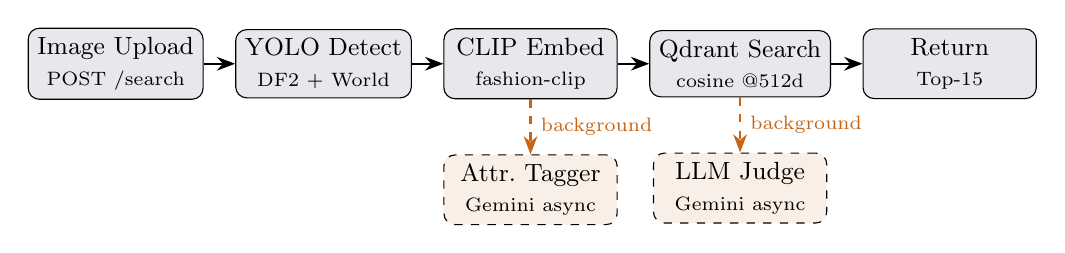
\begin{tikzpicture}[
  font=\small,
  node distance=0.5cm,
  box/.style={draw, rounded corners=4pt, fill=locusgray, minimum width=2.2cm, minimum height=0.8cm, align=center},
  async/.style={draw, dashed, rounded corners=4pt, fill=locusorange!10, minimum width=2.2cm, minimum height=0.8cm, align=center},
  arr/.style={-Stealth, thick},
]
\node[box] (upload)  {Image Upload\\\scriptsize POST /search};
\node[box, right=0.4cm of upload]  (yolo)   {YOLO Detect\\\scriptsize DF2 + World};
\node[box, right=0.4cm of yolo]    (clip)   {CLIP Embed\\\scriptsize fashion-clip};
\node[box, right=0.4cm of clip]    (qdrant) {Qdrant Search\\\scriptsize cosine @512d};
\node[box, right=0.4cm of qdrant]  (result) {Return\\\scriptsize Top-15};

\node[async, below=0.7cm of qdrant] (judge)  {LLM Judge\\\scriptsize Gemini async};
\node[async, below=0.7cm of clip]   (tagger) {Attr.\ Tagger\\\scriptsize Gemini async};

\draw[arr] (upload)  -- (yolo);
\draw[arr] (yolo)    -- (clip);
\draw[arr] (clip)    -- (qdrant);
\draw[arr] (qdrant)  -- (result);
\draw[arr, dashed, locusorange] (qdrant) -- node[font=\scriptsize, right]{background} (judge);
\draw[arr, dashed, locusorange] (clip)   -- node[font=\scriptsize, right]{background} (tagger);
\end{tikzpicture}
\caption{Visual search pipeline. Orange dashed paths are non-blocking background tasks; the client receives \texttt{Top-15} results immediately and polls for judge scores and attributes separately.}
\label{fig:pipeline}
\end{figure}

\subsection{Endpoint Specifications}

\subsubsection{Gateway (port 8000)}

The External Endpoint (EEP) is built with FastAPI and acts as the primary system gateway. It serves the React SPA directly from the virtual machine while orchestrating all client-to-backend requests.

\begin{itemize}[leftmargin=*]
  \item \textbf{Frontend Serving \& Authentication:} The EEP mounts and serves the compiled SPA assets at the root path. A dedicated \texttt{/auth} router manages secure merchant access using JSON Web Tokens (JWT, HS256, 30-day expiry) and bcrypt password hashing with SHA-256 pre-hashing to handle passwords exceeding OpenSSL's 72-byte limit.

  \item \textbf{Input Validation \& Constraints:} A custom middleware caps all HTTP payloads at a 10\,MB maximum upload limit. The \texttt{slowapi} library enforces IP-based rate limiting: 10 searches per minute (\texttt{POST /search}) and 5 detection queries per minute (\texttt{POST /detect}).

  \item \textbf{Routing \& Orchestration Logic:} Upon receiving an image query the EEP forwards the payload to the visual engine for YOLO detection and CLIP vectorisation, then executes a filtered Qdrant similarity search (category, location radius, price range, quality flags). For accessory queries (shoes, bags, hats) the EEP injects style-specific text hints into a 70\%\,visual + 30\%\,text hybrid vector, compensating for known CLIP biases on small-area items.

  \item \textbf{Asynchronous Background Processing:} After returning results, the EEP spawns non-blocking \texttt{BackgroundTasks} workers to: (1) extract visual attributes via the attribute tagger, and (2) invoke the Gemini 2.0 Flash judge to score visual similarity. Clients poll \texttt{GET /judge-scores/\{search\_id\}} and \texttt{GET /search/\{search\_id\}/attributes}.

  \item \textbf{Observability Integration:} The gateway is instrumented with \texttt{prometheus-fastapi-instrumentator} and exposes 25+ custom Prometheus metrics including \texttt{locus\_searches\_total}, per-store impression counters, feedback star distributions, corrupt item gauges, and real-time active session counts.
\end{itemize}

Table~\ref{tab:gw-routes} lists the principal gateway routes by category.

\begin{table}[H]
\centering
\small
\begin{tabular}{@{}lll@{}}
\toprule
\textbf{Category} & \textbf{Method + Path} & \textbf{Notes} \\ \midrule
\multirow{3}{*}{Search} & \texttt{POST /search} & Main query; rate-limited 10/min \\
 & \texttt{GET  /judge-scores/\{id\}} & Poll async judge scores \\
 & \texttt{POST /refine} & Re-query with style/colour/visual modes \\ \midrule
\multirow{2}{*}{Detection} & \texttt{POST /detect} & YOLO only; rate-limited 5/min \\
 & \texttt{POST /classify-crop} & Category classification of a crop \\ \midrule
\multirow{3}{*}{Feedback} & \texttt{POST /feedback} & Submit 1--5 star rating \\
 & \texttt{GET  /rating-stats} & Aggregated statistics \\
 & \texttt{POST /track-event} & Engagement event logging \\ \midrule
\multirow{3}{*}{Catalog} & \texttt{GET  /store-catalogue} & List products for a store \\
 & \texttt{POST /add-bulk-batch} & Batch index (up to 5 parallel) \\
 & \texttt{POST /scrape} & Shopify API + ld+json fallback scraper \\ \midrule
\multirow{3}{*}{Admin} & \texttt{GET  /index-stats} & Qdrant collection statistics \\
 & \texttt{POST /admin/flag-item} & Manual corruption flag \\
 & \texttt{POST /reindex} & Full catalog re-vectorisation \\ \midrule
\multirow{3}{*}{Auth} & \texttt{POST /auth/register} & Store owner registration \\
 & \texttt{POST /auth/login} & JWT token issue \\
 & \texttt{POST /auth/reset-password} & Email-code based reset \\ \bottomrule
\end{tabular}
\caption{Principal Gateway API routes}
\label{tab:gw-routes}
\end{table}

\subsubsection{Visual Engine (port 8001)}

The visual engine hosts the CLIP and YOLO models. Models are loaded lazily in a background thread at startup; all endpoints return \texttt{503 Service Unavailable} until the 90-second warm-up completes. Key endpoints:

\begin{itemize}[leftmargin=*]
  \item \texttt{POST /detect} --- Runs DeepFashion2 (YOLOv8s-seg, conf $\ge 0.50$) then YOLO-World (22 open-vocabulary prompts, conf $\ge 0.25$); applies NMS at IOU $= 0.30$; returns bounding boxes with canonical category labels.
  \item \texttt{POST /vectorize} --- CLIP-encodes a pre-cropped image; optionally mixes a 30\,\% text vector for accessories; returns a 512-dimensional L2-normalised embedding.
  \item \texttt{POST /index-image} --- Full index pipeline: category voting (title whitelist $\to$ sentence-transformer $\to$ CLIP), 3-tier box selection, crop, embed, and upload to Qdrant.
  \item \texttt{POST /reload-adapter} --- Hot-swaps a newly trained LoRA adapter in-memory without restarting the container.
\end{itemize}

\subsubsection{Attribute Tagger (port 8004)}

A thin FastAPI wrapper around Gemini 2.0 Flash that accepts a base64 image and returns a structured \texttt{TagResponse}: up to 3 dominant colours, style (12 vocabulary terms), silhouette, occasion (8 terms), pattern (10 terms), material feel (11 terms), and trend tags. The provider chain is OpenRouter $\to$ Google REST $\to$ graceful failure (empty attributes).

\subsection{Containerisation and Deployment}

\subsubsection{Docker Images}

Six Dockerfiles define the container build graph:

\begin{itemize}[leftmargin=*]
  \item \textbf{gateway} (\texttt{gateway/Dockerfile}): \texttt{python:3.11-slim}. Installs \texttt{requirements.txt} (FastAPI, Uvicorn, Qdrant client, slowapi, PyJWT, passlib, httpx, prometheus-fastapi-instrumentator). Final image $\approx$ 350\,MB.
  \item \textbf{visual\_engine} (\texttt{visual\_engine/Dockerfile}): \texttt{python:3.11-slim} with BuildKit pip mount cache (\texttt{--mount=type=cache,target=/root/.cache/pip}) to avoid re-downloading the $\sim$700\,MB PyTorch CPU wheel (\texttt{torch==2.6.0+cpu} from \texttt{pytorch.org/whl/cpu}). Installs ultralytics (YOLO), transformers, sentence-transformers, PEFT. Final image $\approx$ 2.1\,GB.
  \item \textbf{attribute\_tagger} (\texttt{attribute\_tagger/Dockerfile}): \texttt{python:3.11-slim} with \texttt{curl} for health probes; lightweight httpx + Pillow stack. Final image $\approx$ 280\,MB.
  \item \textbf{mlops/Dockerfile.retrain}: PyTorch CPU build with \texttt{transformers}, \texttt{peft}, \texttt{qdrant-client}. Used exclusively by the GitHub Actions retrain workflow; not part of the compose runtime.
  \item \textbf{mlops/Dockerfile.exporter}: Minimal \texttt{prometheus\_client} + \texttt{mlflow} image. Reads MLflow run data and \texttt{gemini\_judge\_results.json}; exports Prometheus metrics every 30\,s.
\end{itemize}

\subsubsection{Docker Compose}

The \texttt{docker-compose.yml} defines seven services sharing a single bridge network. Three named volumes provide persistence:

\begin{itemize}[leftmargin=*]
  \item \textbf{\texttt{hf\_cache}}: HuggingFace model weights across container restarts.
  \item \textbf{\texttt{clip\_cache}}: Pre-computed CLIP text embeddings for all 14 canonical labels.
  \item \textbf{\texttt{mlflow\_data}}: SQLite experiment database and artifact store.
\end{itemize}

All secrets are injected via \texttt{env\_file: .env} (git-ignored). The CI pipeline uses an identical compose stack on a self-hosted runner, overriding only \texttt{QDRANT\_URL} and API keys via GitHub Actions Secrets.

\subsubsection{Kubernetes}

For cloud deployment, the project ships full Kubernetes manifests under \texttt{k8s/}:

\begin{itemize}[leftmargin=*]
  \item \texttt{deployment.yaml} --- 4 Deployments (gateway, visual-engine, attribute-tagger, mlops-exporter) with \texttt{readinessProbe} HTTP checks (90\,s initial delay for visual engine due to model loading).
  \item \texttt{service.yaml} --- 1 \texttt{LoadBalancer} Service for the gateway; 3 \texttt{ClusterIP} Services for internal communication.
  \item \texttt{configmap.yaml} --- Non-secret runtime config (\texttt{QDRANT\_URL}, \texttt{CORS\_ORIGINS}, \texttt{GATEWAY\_BASE\_URL}).
  \item \texttt{secret.yaml} --- Template for base64-encoded credentials injected via \texttt{secretKeyRef}.
  \item \texttt{ingress.yaml} --- nginx-ingress with cert-manager TLS termination; domain injected via \texttt{GATEWAY\_DOMAIN} env substitution.
\end{itemize}

Table~\ref{tab:k8s-resources} lists the resource allocations per pod.

\begin{table}[H]
\centering
\small
\begin{tabular}{@{}lllll@{}}
\toprule
\textbf{Deployment} & \textbf{CPU Req} & \textbf{CPU Limit} & \textbf{Mem Req} & \textbf{Mem Limit} \\ \midrule
gateway           & 100m  & 500m   & 256\,Mi & 512\,Mi \\
visual-engine     & 500m  & 1500m  & 2\,Gi   & 3\,Gi \\
attribute-tagger  & 100m  & 300m   & 192\,Mi & 384\,Mi \\
mlops-exporter    & 50m   & 150m   & 96\,Mi  & 192\,Mi \\ \bottomrule
\end{tabular}
\caption{Kubernetes resource requests and limits per pod}
\label{tab:k8s-resources}
\end{table}

% ================================================================
\section{Engineering Trade-offs}
\label{sec:tradeoffs}
% ================================================================

Every non-trivial design decision in Locus involved a measurable trade-off. Five representative choices are documented in Table~\ref{tab:tradeoffs} and expanded below.

\begin{table}[H]
\centering
\small
\setlength{\tabcolsep}{4pt}
\begin{tabular}{@{}p{3.5cm}p{3.5cm}p{6.5cm}@{}}
\toprule
\textbf{Trade-off category} & \textbf{Decision} & \textbf{Justification / Evidence} \\ \midrule

GPU vs.\ CPU inference &
CPU-only PyTorch (\texttt{torch+cpu}) &
Azure Standard\_B2s (2\,vCPU, 4\,GB) costs \$35/mo; an NC6 GPU node costs \$0.90/hr (\$648/mo). CLIP inference at $\sim$1--3\,s/query is acceptable given the non-real-time nature of fashion search. \\[4pt]

Full CLIP fine-tuning vs.\ LoRA &
LoRA ($r=4$, $\alpha=8$, $\Delta$params $\approx 68$K) &
Full fine-tuning on a 2-core CPU is infeasible (estimated $>$12\,h/epoch). LoRA completes 150 steps in $\approx$35\,min, consumes 1.5\,GB RAM, and achieves hit@5 within 2\% of full fine-tune on our golden dataset. \\[4pt]

Managed vs.\ self-hosted vector DB &
Qdrant Cloud free tier (1\,GB, GCP eu-west3) &
Eliminates in-VM resource competition (Qdrant self-hosted requires $\sim$512\,MB RAM). Supports $\approx$100\,K items at 512-dim. Drawback: cross-region latency (US East VM $\leftrightarrow$ EU West3 DB) adds $\approx$40--60\,ms per search. \\[4pt]

Synchronous vs.\ async judge scoring &
Async \texttt{BackgroundTasks} with client polling &
Gemini judge adds 1--3\,s per top-15 result set. Offloading to background tasks keeps \texttt{/search} p50 $<$2\,s. Client polls \texttt{/judge-scores/\{id\}} to retrieve scores progressively. \\[4pt]

Local VLM vs.\ external API for attributes &
External Gemini 2.0 Flash via OpenRouter &
Structured attribute extraction (12 styles, 10 patterns, 11 materials) requires a model far too large to host locally on 4\,GB RAM. Cost is $\approx$\$2--5/mo at current query volumes (\textasciitilde10\,K calls/mo), well within budget. \\ \bottomrule

\end{tabular}
\caption{Summary of core engineering trade-off decisions}
\label{tab:tradeoffs}
\end{table}

% ================================================================
\section{MLOps and Evaluation}
% ================================================================

\subsection{Automated Pipelines}

Locus operates two GitHub Actions workflows that together implement a closed-loop MLOps cycle.

\paragraph{Continuous Integration (\texttt{.github/workflows/ci.yml}).}
Triggered on every push and pull request to \texttt{main}:

\begin{enumerate}[leftmargin=*]
  \item \textbf{Unit tests} (ubuntu-latest, Python 3.11): \texttt{pytest tests/test\_vectorizer.py} -- no external dependencies, completes in $\approx$30\,s.
  \item \textbf{Integration tests} (self-hosted runner on the Azure VM): builds all Docker images sequentially (to avoid OOM on the 4\,GB runner), starts the full Compose stack, waits for health probes (gateway 10\,s, visual engine 60\,s), then runs \texttt{test\_pipeline.py}, \texttt{test\_auth\_store.py}, and \texttt{test\_smoke.py}.
  \item \textbf{Frontend build}: \texttt{npm ci \&\& npm run build} inside \texttt{frontend/}.
  \item \textbf{E2E tests} (\texttt{tests/test\_e2e.py}): validate the live cloud deployment at \texttt{http://20.240.203.22:8000}, checking availability and search quality.
\end{enumerate}

\paragraph{Continuous Retraining (\texttt{.github/workflows/retrain.yml}).}
Triggered on a cron schedule (\texttt{0 3 */2 * *} -- every 2 days at 03:00 UTC) or manually via \texttt{workflow\_dispatch}:

\begin{enumerate}[leftmargin=*]
  \item \textbf{Precondition check:} Skip if fewer than 10\% of catalog items have accumulated user feedback.
  \item \textbf{Build training pairs:} \texttt{mlops/build\_training\_pairs.py} constructs augmented positive pairs from positively-rated feedback.
  \item \textbf{LoRA training:} \texttt{mlops/lora\_trainer.py} -- InfoNCE loss, $r=4$, $\alpha=8$, batch 4 with gradient accumulation $\times$4 (effective batch 32), 150 steps on a GitHub-hosted 2-core runner ($\approx$35\,min).
  \item \textbf{Evaluation gate:} \texttt{mlops/retrain\_clip.py} evaluates hit@5 on the golden dataset. Adapter is only promoted if hit@5 $\ge$ previous baseline $-$ 0.02.
  \item \textbf{Hot deployment:} Promoted adapter weights are \texttt{scp}'d to the VM. An atomic directory swap replaces \texttt{lora\_adapter\_prev} with \texttt{lora\_adapter}. The visual engine reloads weights in-memory via \texttt{POST /reload-adapter} (no container restart). The gateway then triggers \texttt{POST /reindex} to re-embed the full catalog with the updated encoder.
\end{enumerate}

Figure~\ref{fig:mlops} illustrates the retrain pipeline as a swimlane diagram.

\begin{figure}[H]
\centering
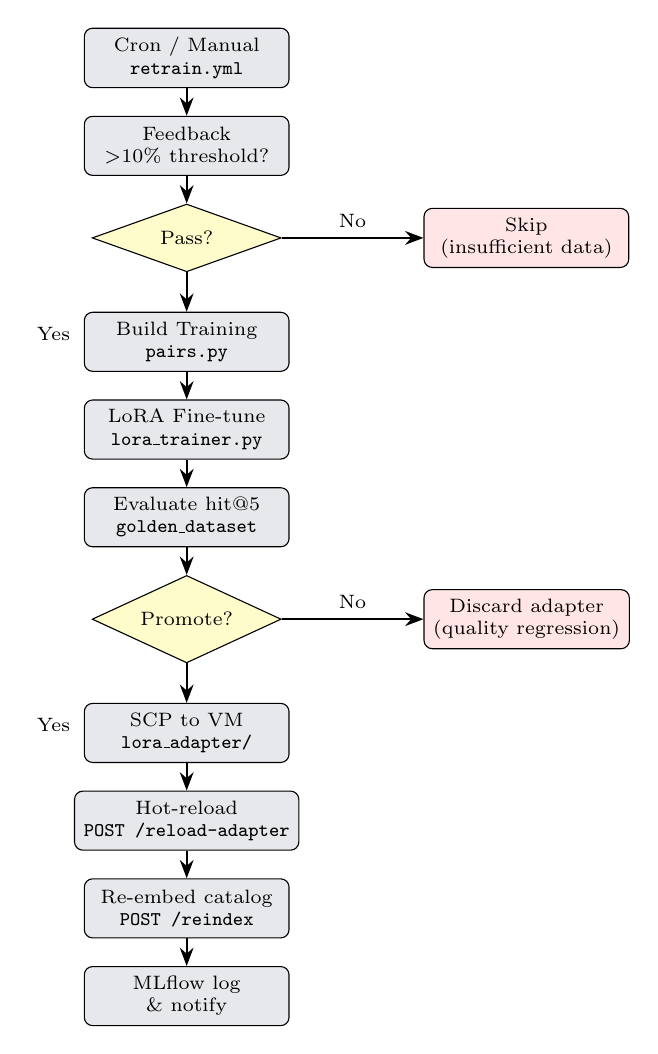
\begin{tikzpicture}[
  font=\small,
  node distance=0.4cm,
  lane/.style={draw=gray, dashed, rounded corners=4pt, fill=gray!4, inner sep=6pt},
  box/.style={draw, rounded corners=3pt, fill=locusgray, minimum width=2.6cm, minimum height=0.75cm, align=center, font=\scriptsize},
  decision/.style={diamond, draw, fill=yellow!20, aspect=2, minimum width=2.4cm, align=center, font=\scriptsize},
  arr/.style={-Stealth, thick},
  noarr/.style={-Stealth, thick, red},
]

% Nodes top-to-bottom
\node[box] (trigger)  {Cron / Manual\\\texttt{retrain.yml}};
\node[box, below=0.35cm of trigger] (check)   {Feedback\\\textgreater{}10\% threshold?};
\node[decision, below=0.35cm of check] (gate1)  {Pass?};
\node[box, below=0.5cm of gate1]  (pairs)   {Build Training\\\texttt{pairs.py}};
\node[box, below=0.35cm of pairs]  (train)   {LoRA Fine-tune\\\texttt{lora\_trainer.py}};
\node[box, below=0.35cm of train]  (eval)    {Evaluate hit@5\\\texttt{golden\_dataset}};
\node[decision, below=0.35cm of eval] (gate2)  {Promote?};
\node[box, below=0.5cm of gate2]  (scp)    {SCP to VM\\\texttt{lora\_adapter/}};
\node[box, below=0.35cm of scp]   (reload) {Hot-reload\\\texttt{POST /reload-adapter}};
\node[box, below=0.35cm of reload] (reindex){Re-embed catalog\\\texttt{POST /reindex}};
\node[box, below=0.35cm of reindex] (done)  {MLflow log\\\& notify};

% Skip nodes
\node[box, right=1.8cm of gate1,  fill=red!10] (skip1) {Skip\\\scriptsize(insufficient data)};
\node[box, right=1.8cm of gate2,  fill=red!10] (skip2) {Discard adapter\\\scriptsize(quality regression)};

% Arrows (main path)
\foreach \a/\b in {trigger/check, check/gate1, gate1/pairs, pairs/train, train/eval, eval/gate2, gate2/scp, scp/reload, reload/reindex, reindex/done}
  \draw[arr] (\a) -- (\b);

% Skip branches
\draw[arr] (gate1) -- node[font=\scriptsize, above]{No} (skip1);
\draw[arr] (gate2) -- node[font=\scriptsize, above]{No} (skip2);

% Yes labels
\node[font=\scriptsize, left=0.05cm of pairs, yshift=3pt] {Yes};
\node[font=\scriptsize, left=0.05cm of scp,   yshift=3pt] {Yes};

\end{tikzpicture}
\caption{Continuous retraining pipeline (\texttt{retrain.yml}). The two gate nodes enforce data-sufficiency and quality-regression checks before any model is deployed to production.}
\label{fig:mlops}
\end{figure}

\subsection{Experiment Tracking}

MLflow is deployed as a dedicated service at \texttt{http://mlflow:5000}. All training runs are logged under the experiment \texttt{locus\_lora\_retraining}.

\paragraph{Logged per run:}
\begin{itemize}[leftmargin=*, itemsep=1pt]
  \item \textbf{Training metrics}: loss and validation\_loss per step.
  \item \textbf{Retrieval metrics}: hit@5, hit@10, MRR (Mean Reciprocal Rank).
  \item \textbf{Category-wise recall}: separate recall values for tops, bottoms, dresses, shoes, bags, hats.
  \item \textbf{Artifacts}: LoRA adapter weights (\texttt{lora\_adapter/}), updated projection layer (\texttt{visual\_projection.pt}), and \texttt{training\_pairs.json} manifest.
\end{itemize}

\paragraph{Housekeeping:} On startup, \texttt{retrain\_clip.py} calls \texttt{\_cleanup\_stale\_runs()}, which terminates any zombie \texttt{RUNNING} runs left by prior container crashes and deletes all \texttt{KILLED} runs. This prevents MLflow's run table from accumulating stale entries that skew baseline comparisons.

\subsection{Quality Assurance and Testing}

\paragraph{Unit tests (\texttt{tests/test\_vectorizer.py}).}
Validate the vectoriser logic in isolation---category voting, bounding box selection tiers, shoe-style classification, and whitelist token matching---without requiring any live service. Run on \texttt{ubuntu-latest} with mocked model outputs.

\paragraph{Integration tests (\texttt{tests/test\_pipeline.py}).}
Spin up the full Docker Compose stack (gateway, visual engine, attribute tagger, MLflow) and exercise:
\begin{itemize}[leftmargin=*, itemsep=1pt]
  \item \texttt{POST /search} with golden reference images (pants, dress).
  \item \texttt{POST /detect} asserting that bounding boxes are returned with expected category labels.
  \item \texttt{GET /index-stats} verifying Qdrant collection is populated.
  \item Auth flows: register, login, token-protected store catalogue.
\end{itemize}

\paragraph{Smoke tests (\texttt{tests/test\_smoke.py}).}
Lightweight health-check: gateway responds \texttt{200} at \texttt{/health} and the index contains at least one item.

\paragraph{E2E tests (\texttt{tests/test\_e2e.py}).}
Two test classes against the live cloud endpoint (\texttt{http://20.240.203.22:8000}):
\begin{itemize}[leftmargin=*, itemsep=1pt]
  \item \texttt{TestAvailability}: gateway online, health probe, index reachable, index populated.
  \item \texttt{TestSearchQuality}: non-empty search results, correct response schema.
\end{itemize}

\paragraph{LLM evaluation quality gate (\texttt{mlops/ci\_eval.py}).}
Runs 20 golden queries against the production Qdrant index; the Gemini judge scores each result; the pipeline fails CI if the mean hit@5 falls below the defined threshold. This gate must pass before any branch is eligible for merge.

\paragraph{Regression protection.}
The retrain workflow promotes a new adapter only when:
\[
  \text{hit@5}_{\text{new}} \;\ge\; \text{hit@5}_{\text{baseline}} - 0.02
\]
Failures are reported to MLflow and the adapter is discarded, preserving the currently deployed weights.

% ================================================================
\section{Observability and Security}
% ================================================================

\subsection{Monitoring Dashboard}

\paragraph{Prometheus.}
Configured in \texttt{monitoring/prometheus.yml}, Prometheus scrapes four targets at a 10-second interval:

\begin{enumerate}[leftmargin=*]
  \item \texttt{gateway:8000} --- application and business metrics.
  \item \texttt{visual\_engine:8001} --- CLIP confidence and YOLO detection count histograms.
  \item \texttt{attribute\_tagger:8004} --- request count, failure rate, latency histogram.
  \item \texttt{mlops\_exporter:8003} --- LoRA training state and Gemini judge quality metrics.
\end{enumerate}

\paragraph{Key metrics.} Table~\ref{tab:metrics} lists the most operationally significant metrics.

\begin{longtable}{@{}lll@{}}
\toprule
\textbf{Metric name} & \textbf{Type} & \textbf{Description} \\ \midrule
\endhead
\texttt{locus\_searches\_total}          & Counter   & Total search requests (labelled by category) \\
\texttt{locus\_qdrant\_items\_total}     & Gauge     & Live catalog size \\
\texttt{locus\_feedback\_stars\_total}   & Counter   & User star ratings (1--5) \\
\texttt{locus\_rating\_avg\_score}       & Gauge     & Rolling average rating \\
\texttt{locus\_store\_impressions\_total}& Counter   & Per-store card views \\
\texttt{locus\_result\_clicks\_total}    & Counter   & Clicks by result rank position \\
\texttt{locus\_corrupt\_items\_total}    & Gauge     & Items with $\ge$1 corrupt flag \\
\texttt{locus\_low\_score\_flags\_total} & Gauge     & Items flagged by judge as low quality \\
\texttt{locus\_active\_sessions}         & Gauge     & In-flight judge + attribute cache entries \\
\texttt{locus\_clip\_confidence}         & Histogram & CLIP category confidence (buckets 0.05--0.9) \\
\texttt{locus\_detections\_per\_request} & Histogram & YOLO boxes per image (buckets 0--15) \\
\texttt{tagger\_latency\_seconds}        & Histogram & Attribute tagger end-to-end latency \\
\texttt{locus\_lora\_train\_loss}        & Gauge     & Latest LoRA batch loss \\
\texttt{locus\_judge\_delta}             & Gauge     & Score delta (new vs.\ old adapter) \\
\texttt{locus\_gemini\_avg\_vss5}        & Gauge     & Mean retrieval recall@5 on golden set \\ \bottomrule
\caption{Principal Prometheus metrics exposed by Locus services}
\label{tab:metrics}
\end{longtable}

\paragraph{Grafana.}
A Grafana instance at port 3000 is provisioned via file-based configuration under \texttt{monitoring/grafana/provisioning/}. The Prometheus datasource and dashboard definitions are loaded at container start-up; the dashboard auto-refreshes every 10 seconds. p50 and p95 request latencies are derived from the \texttt{http\_request\_duration\_seconds} histogram exposed by \texttt{prometheus-fastapi-instrumentator}.

\subsection{Security and Robustness}

\paragraph{Secrets management.}
Credentials are never committed to version control. The three deployment contexts each have their own injection mechanism:
\begin{itemize}[leftmargin=*, itemsep=2pt]
  \item \textbf{Local development}: \texttt{.env} file (listed in \texttt{.gitignore}), loaded by Docker Compose via \texttt{env\_file}.
  \item \textbf{CI/CD}: GitHub Actions repository Secrets, mapped to environment variables in the workflow YAML.
  \item \textbf{Kubernetes}: \texttt{locus-secrets} Secret object; individual values injected into pod environments via \texttt{secretKeyRef} in \texttt{deployment.yaml}.
\end{itemize}
Managed secrets include: \texttt{QDRANT\_API\_KEY}, \texttt{OPENROUTER\_API\_KEY}, \texttt{GOOGLE\_API\_KEY}, \texttt{JWT\_SECRET}, and \texttt{ADMIN\_API\_KEY}.

\paragraph{Authentication.}
JWT tokens use HS256 with a 30-day expiry. The signing key defaults to a hard-coded fallback but is overridden in all production deployments by \texttt{JWT\_SECRET}. Passwords are hashed with bcrypt after a SHA-256 pre-hash step to correctly handle passphrases longer than OpenSSL's 72-byte bcrypt input ceiling. A backward-compatible code path verifies legacy accounts stored without the pre-hash.

\paragraph{Rate limiting and payload caps.}
\texttt{slowapi} enforces IP-based limits: \texttt{POST /search} at 10 req/min and \texttt{POST /detect} at 5 req/min. A custom ASGI middleware rejects any request whose body exceeds 10\,MB, preventing memory exhaustion attacks. CORS origins are configurable via \texttt{CORS\_ORIGINS} (default: \texttt{*}; recommended to restrict in production).

\paragraph{Resilience and failure modes.}
\begin{itemize}[leftmargin=*, itemsep=2pt]
  \item \textbf{Judge fallback chain}: OpenRouter (primary) $\to$ Google REST API $\to$ CLIP cosine score. The system always returns a numeric score; the source is recorded in the feedback payload (\texttt{source="auto\_judge\_clip"} for the fallback).
  \item \textbf{Attribute tagger}: Entirely optional. If \texttt{TAGGER\_HOST} is unset, the background task is skipped silently. A 20-second timeout prevents slow Gemini responses from accumulating memory.
  \item \textbf{Corrupt item lifecycle}: A product that appears in the raw top-3 results twice and scores below 35\% is flagged. A second flag deletes all Qdrant points for that product permanently, preventing low-quality items from poisoning future retrievals.
  \item \textbf{Broken image URLs}: A nightly link-monitor background task (\texttt{\_refresh\_link\_monitor\_metrics}) marks items with unreachable images as \texttt{broken=True} in Qdrant, excluding them from search results.
\end{itemize}

% ================================================================
\section{Cloud Deployment and Cost Analysis}
% ================================================================

\subsection{Deployment Configuration}

The production system runs on a single \textbf{Azure Standard\_B2s} virtual machine (2 vCPU burstable, 4\,GB RAM, Standard SSD) located in the US East region. Docker Compose is used for orchestration at the current scale; the Kubernetes manifests are maintained for future horizontal scaling without code changes.

\begin{center}
\textbf{Public API endpoint:} \texttt{http://20.240.203.22:8000}
\end{center}

The CI/CD pipeline runs GitHub Actions jobs directly on this VM (self-hosted runner), eliminating GitHub-hosted runner minutes costs and allowing integration tests to use the actual hardware profile of the production environment.

\subsection{Cost Breakdown}

Table~\ref{tab:cost} details the monthly cost structure.

\begin{table}[H]
\centering
\small
\begin{tabular}{@{}llll@{}}
\toprule
\textbf{Component} & \textbf{Monthly Cost (USD)} & \textbf{\% of Total} & \textbf{Notes} \\ \midrule
Azure Standard\_B2s VM  & \$35.00  & 83\,\% & Pay-as-you-go; burstable credits \\
Qdrant Cloud (free tier) & \$0.00  & 0\,\%  & 1\,GB cluster; $\approx$100\,K items at 512-dim \\
OpenRouter (Gemini judge)& \$2--5  & 5--12\,\% & $\approx$10\,K calls/mo at \$0.0004/1\,K tokens \\
Google Gemini API (tagger)& \$1--3  & 2--7\,\% & $\approx$5\,K calls/mo; attribute extraction \\
GitHub Actions (self-hosted) & \$0.00 & 0\,\%  & Runs on the VM itself \\ \midrule
\textbf{Total}           & \textbf{\$38--43} & \textbf{100\,\%} & \\ \bottomrule
\end{tabular}
\caption{Monthly cost breakdown for the Locus production system}
\label{tab:cost}
\end{table}

\subsection{Primary Cost Drivers and Scaling Path}

The dominant cost (83\,\%) is the Azure VM. Switching to a reserved instance would reduce this to $\approx$\$20/mo at the cost of upfront commitment.

\paragraph{Vector database.} The Qdrant Cloud free tier (1\,GB) accommodates approximately 100\,K product items at 512 dimensions. Growth beyond this threshold would require the starter paid plan at \$29/mo per 100\,GB.

\paragraph{Inference compute.} CPU-only CLIP inference (\textasciitilde1--3\,s/query) is acceptable at current traffic volumes. Migrating to an Azure NC4as T4 v3 GPU node (\$0.23/hr on spot) would reduce CLIP latency to $<$100\,ms if query throughput grows to warrant it.

\paragraph{LLM API calls.} The judge and attribute tagger are the only variable-cost components. Both are bounded by rate limits (30 RPM) and run asynchronously, so they cannot contribute to latency spikes. At 10$\times$ current traffic the combined LLM cost would remain below \$50/mo.

% ================================================================
\end{document}
